\section{Time Series}
\begin{definition}[Time series]
A \textbf{time series}  $T = \{t_1, \dots,t_c\}$ is a collection of $c$ signals, each one with $m$ observations $x_i$, i.e. $t_j = \{x_1, \dots, x_m\}$ made sequentially in time. It is \textbf{univariate} if $c = 1$ and  \textbf{multivariate} if $c > 1$.
\end{definition}

\begin{definition}
    {Time series data}
    A \textbf{time series dataset} is a collection of time series $X = \{T_1,...,T_n\}$. Each time series $T_i$ may carry exogenous variables (\textit{categorical} or \textit{continuous}).
\end{definition}
Given a dataset $X = \{T_1, \dots, T_n\}$, we distinguish several tasks.
\begin{itemize}
    \item \textbf{Time series classification (TSC):} aims to train a model $f$ to predict an \textbf{exogenous} \textbf{categorical} output $y$ for each $T_i$.
    \item \textbf{Time Series extrinsic regression (TSER)}: aims to train a model $f$ to predict an \textbf{exogenous} \textbf{continuous} output $y_i$ for each time series $T_i$.
    \item \textbf{Time series forecasting (TSF):} aims to train a model $f$ to predict an \textbf{endogenous continuous} output $y$ for each time series $T$.
    \item \textbf{Time series clustering (TSC):} aims to group similar time series into clusters.
    \item \textbf{Anomaly detection:} aims to identify anomalous time series within the set $X$, or anomalous time stamps within each time series $T$.
    \item \textbf{Pattern mining:} aims to identify repeated subsequences in each time series $T$.
\end{itemize}

\paragraph{Important Assumption} We assume that, given $X= \{T_1, \dots, T_n\}$, all the time series have aligned time stamps: the $i$-th time step of a time series $T_a$ corresponds to the $i$-th time step of another time series $T_b$, and this holds for every pair in $X$.

\subsection{Visualization}
A plot can reveal:
\begin{itemize}
    \item \textbf{Trend}: upward or downward pattern
    \item \textbf{Periodicity}: repetition of behavior in a regular pattern
    \item \textbf{Seasonality}: periodic behavior with a known period (hourly, weekly, monthly...)
    \item \textbf{Heteroskedasticity}: changing variance
    \item \textbf{Dependence}: positive (successive observations are similar) or negative (successive observations are dissimilar)
    \item \textbf{Outliers}: anomalous time stamps, anomalous subsequences
    \item \textbf{Missing data}: missing values at a certain time stamp or longer subsequences
\end{itemize}

\textit{\textbf{Note}: $K$-means clustering with medoid visualization provides a meaningful, reduced subset of representative time series.}
\subsection{Handling Missing Values}
Individual or contiguous values in a time series can be missing. We deal with them in several ways:
\begin{itemize}
    \item Fill with a constant value:
    \begin{itemize}
        \item last value (\textit{pad})
        \item next value (\textit{backfill})
        \item \textit{mean/median} value
        \item \textit{nearest value}
    \end{itemize}
    \item linear interpolation:
    \begin{itemize}
        \item interpolate between the last and first non-missing values to recover the missing ones.
    \end{itemize}
    \item forecasting:
    \begin{itemize}
        \item fill using a forecasting or regressive model.
    \end{itemize}
    \item random.
\end{itemize}

\subsection{Anomalies}
Outlier detection methods differ depending on the type of outlier:
\begin{itemize}
    \item \textbf{Point outlier}: a value that behaves unusually at a specific time instant when compared either to the other values in the time series (global outlier) or to its neighboring points (local outlier).
    \item \textbf{Subsequence}: consecutive points in time whose joint behavior is unusual, although each observation individually is not necessarily a point outlier.
    \item Entire time series can also be outliers, but they can only be detected when the input is a dataset of time series.
\end{itemize}

An outlier is a point that significantly deviates from its expected value.

Given a univariate time series $x$, a point $t$ is declared an outlier if the distance to its expected value is higher than a predefined threshold.
\begin{itemize}
    \item \textbf{estimation method}: $\overline x_t$ is obtained using observations both before and after $x_t$ (past, current and future data).
    \item \textbf{prediction method}: $\overline x_t$ is obtained relying only on observations before $x_t$ (past data).
\end{itemize}

\subsubsection{Data Visualization for Outlier Detection}

\paragraph{Histogram} A histogram gives a visual representation of the data distribution, letting us identify potential outliers that fall outside the main distribution pattern.

\begin{itemize}
    \item The x-axis represents data values divided into bins
    \item The y-axis represents the frequency (count) of observations in each bin
    \item Observations far from the main distribution (in the tails) are potential outliers
\end{itemize}

\paragraph{Boxplot} A boxplot is a standardized way of displaying the distribution of data based on a five-number summary: minimum, first quartile (Q1), median, third quartile (Q3), and maximum.

\subsubsection{Outlier Detection Methods}

\paragraph{Inter-Quartile Range (IQR) Filter} Values that fall
\begin{itemize}
    \item above Q3 + 1.5 * IQR, or
    \item below Q1 - 1.5 * IQR
\end{itemize}
are considered potential outliers. Here Q3 and Q1 are the third ($q_{0.75}$) and first ($q_{0.25}$) quartile respectively, and IQR is the difference between the third and first quartile.

\begin{equation}
\text{Potential outliers} = \{x | x < Q1 - 1.5 \cdot IQR \text{ or } x > Q3 + 1.5 \cdot IQR\}
\end{equation}

\paragraph{Hampel Filter} The Hampel filter flags as outliers the values outside the interval $I$ formed by the median, plus or minus 3 Median Absolute Deviations (MAD):

\begin{equation}
I = [\text{median}_X - 3 \cdot \text{MAD}; \text{median}_X + 3 \cdot \text{MAD}]
\end{equation}

where MAD is the median absolute deviation and is defined as the median of the absolute deviations from the data's median, i.e.,

\begin{equation}
\text{MAD} = \text{median}(|x_i - \text{median}_X|)
\end{equation}

\paragraph{Grubbs' Test} Grubbs' test detects outliers in univariate data and has the following characteristics:
\begin{itemize}
    \item Assumes data comes from normal distribution
    \item Detects one outlier at a time, removes the outlier, and repeats
    \item H$_0$: There is no outlier in data
    \item H$_A$: There is at least one outlier
\end{itemize}

Grubbs' test statistic: 
\begin{equation}
G = \frac{\max|X - \bar{X}|}{s}
\end{equation}
where $\bar{X}$ is the mean and $s$ is the standard deviation.

Reject null hypothesis H$_0$ of no outliers if:
\begin{equation}
G > \frac{(N-1)}{\sqrt{N}} \sqrt{\frac{t^2_{(\alpha/N, N-2)}}{N-2+t^2_{(\alpha/N, N-2)}}}
\end{equation}

where:
\begin{itemize}
    \item $\alpha$ is the significance level
    \item $t$ is the Student's t-distribution
    \item $N$ is the sample size
    \item For one-sided test, use $\alpha/N$
    \item For two-sided test, use $\alpha/2N$
\end{itemize}

\subsection{Time Series Normalizations}

A common tool of Time Series Analysis (TSA) is computing distances among time series. Several challenges arise:
\begin{itemize}
    \item many Machine Learning (ML) tools require the input data to lie in the same range of values, or at least that the values be comparable;
    \item distance calculations and ML models are very sensitive to distortions in the data, so these distortions should be removed.
\end{itemize}

The most common distortions are:
\begin{itemize}
    \item Offset Translation
    \item Amplitude Scaling
    \item Linear Trend
    \item Presence of Noise
\end{itemize}

These distortions can be removed by using the appropriate normalizations.

\subsubsection{Normalization Techniques}

\paragraph{Offset Translation: Mean Removal}

Mean removal is applied to center the time series around zero:

\begin{equation}
Q = Q - \text{mean}(Q)
\end{equation}
\begin{equation}
C = C - \text{mean}(C)
\end{equation}

This places the time series at the same height on the $y$ axis.

\paragraph{Offset Translation: Min-Max Normalization}

Min-Max normalization scales the time series to range [0,1]:

\begin{equation}
Q = \frac{Q - \min(Q)}{\max(Q) - \min(Q)}
\end{equation}
\begin{equation}
C = \frac{C - \min(C)}{\max(C) - \min(C)}
\end{equation}

\begin{figure}[htbp]
    \centering
    \begin{minipage}{0.32\textwidth}
        \centering
        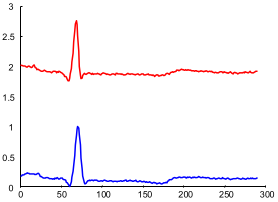
\includegraphics[width=\linewidth]{img/original_TS_mean_minMax.png}
        \caption{Original TS}
        \label{fig:original}
    \end{minipage}
    \hfill
    \begin{minipage}{0.32\textwidth}
        \centering
        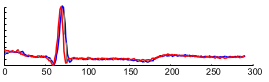
\includegraphics[width=\linewidth]{img/mean_removal_correct.png}
        \caption{mean removal}
        \label{fig:mean-removal}
    \end{minipage}
    \hfill
    \begin{minipage}{0.32\textwidth}
        \centering
        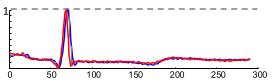
\includegraphics[width=\linewidth]{img/TS_minMax_norm.png}
        \caption{min-max}
        \label{fig:min-max}
    \end{minipage}
\end{figure}
\paragraph{Amplitude Scaling: Z-Score Normalization}

Z-score normalization standardizes the time series to have mean 0 and standard deviation 1:

\begin{equation}
Q = \frac{Q - \text{mean}(Q)}{\text{std}(Q)}
\end{equation}
\begin{equation}
C = \frac{C - \text{mean}(C)}{\text{std}(C)}
\end{equation}

Two time series with different amplitudes before normalization can become comparable after z-score normalization.

\paragraph{Linear Trend: Detrending}

To detrend a time series, fit the best fitting straight line to the time series, then subtract that line from the time series.

\paragraph{Noise Removal: Mean Smoothing}

The intuition behind removing noise is to average each datapoint's value with its neighbors.

\begin{equation}
Q = \text{smooth}(Q)
\end{equation}
\begin{equation}
C = \text{smooth}(C)
\end{equation}

\paragraph{Moving Average}
A Moving Average (MA) is a technique that smooths time series data by creating a new series where each value is the average of a window of consecutive observations from the original series.

Given a window of length $w$ and a time series $t$, the MA is applied as follows:

\begin{equation}
t_i = \frac{1}{w} \sum_{j=i-(w-1)/2}^{i+(w-1)/2} t_j \text{ for } i = 1, ..., n
\end{equation}

For example, if $w=3$ we have:

\begin{equation}
t_i = \frac{1}{3} (t_{i-1} + t_i + t_{i+1})
\end{equation}

\paragraph{Log Transformation}
We apply the logarithm to each value of the time series:

\begin{itemize}
    \item Log:
    \begin{equation}
    Q = \log(Q)
    \end{equation}
    \begin{equation}
    C = \log(C)
    \end{equation}
    
    \item Log1p (useful when data contains zeros):
    \begin{equation}
    Q = \log(Q + 1)
    \end{equation}
    \begin{equation}
    C = \log(C + 1)
    \end{equation}
\end{itemize}

\paragraph{Differencing Transformation}

Differencing: we take the difference of the observation at a particular instant with that at the previous instant.

\begin{equation}
Q = Q_i - Q_{i-1}
\end{equation}
\begin{equation}
C = C_i - C_{i-1}
\end{equation}

\textit{Image slide 72: Left graph shows original time series with strong trends, right graph shows the differenced series which has removed the trends and made the series more stationary.}

\subsection{Time Series Components}

Various Data Mining, Machine Learning and TSA models assume that variables are Independent and Identically Distributed (IID). However, in time series analysis:
\begin{itemize}
    \item Time series values are (usually) not independent
    \item Trend and seasonality might be present
    \item Variance may change significantly (heteroskedasticity)
\end{itemize}

A first goal in TSA is to reduce the time series to a simpler case:
\begin{itemize}
    \item eliminate trend;
    \item eliminate seasonality;
    \item eliminate heteroskedasticity.
\end{itemize}

We then model the remainder as dependent but identically distributed variables.

\subsubsection{Components of Time Series}

A given time series consists of three systematic components, level, trend and seasonality, and one non-systematic component called noise:
\begin{itemize}
    \item \textbf{Level}: The average value in the series.
    \item \textbf{Trend}: The increasing or decreasing value in the series.
    \item \textbf{Seasonality}: The repeating short-term cycle in the series.
    \item \textbf{Noise}: The random variation in the series.
\end{itemize}

A systematic component has consistency or recurrence and can be described and modeled. A non-systematic component cannot be directly modeled.

\subsubsection{Time Series Models}

A time series can be modeled as an aggregate or combination of the four components. All series have a level and noise. The trend and seasonality components are optional. Level can be omitted if Offset Translation with Mean Removal is applied.

\paragraph{Additive Model}
\begin{equation}
Y = \text{Level} + \text{Trend} + \text{Seasonality} + \text{Noise/Residuals}
\end{equation}

Characteristics:
\begin{itemize}
    \item changes over time occur consistently by the same amount;
    \item a linear trend is a straight line;
    \item a linear seasonality keeps the same frequency (width of cycles) and amplitude (height of cycles).
\end{itemize}

\paragraph{Multiplicative Model}
\begin{equation}
Y = \text{Level} \times \text{Trend} \times \text{Seasonality} \times \text{Noise/Residuals}
\end{equation}

Characteristics:
\begin{itemize}
    \item a multiplicative model is nonlinear, such as quadratic or exponential;
    \item changes increase or decrease over time;
    \item a nonlinear trend is a curved line;
    \item a nonlinear seasonality has increasing or decreasing frequency and/or amplitude over time.
\end{itemize}

\subsubsection{Component Meanings}

\begin{itemize}
    \item \textbf{Trend}: upward or downward pattern that might be extrapolated into the future.
    \item \textbf{Seasonality}: periodic behavior with a known period (hourly, weekly, monthly...).
    \item \textbf{Residuals}: containing anything else, i.e., noise.
\end{itemize}

For an additive model:
\begin{equation}
Y = T + S + R
\end{equation}
where Y is the time series, T is trend, S is seasonality, and R is residuals.

\textit{Image slide 77: Four graphs showing decomposition of a time series into: original series Y (top), trend component T (second), seasonal component S (third), and residual component R (bottom).}

\subsubsection{Time Series Decomposition}

\paragraph{Trend}

There are several methods to identify the trend component:
\begin{itemize}
    \item Trend as a straight line between the first and the last point of the time series
    \item Given a window $w$, trend as the moving average along time series with size $w$
    \item Trend as the best fitting straight line obtained with a linear regression
\end{itemize}

\paragraph{Seasonality}

Assume a time series modeled additively, with an estimated period length $p$ and a detrended series $D = Y - T$. Seasonality is then computed per time stamp as the mean value across the successive periods, and this length-$p$ profile is repeated to span the whole series.

\paragraph{Residuals}

Given the time series $Y$, its trend $T$, its seasonality $S$, the residuals $R$ are obtained as:

\begin{equation}
R = Y - T - S
\end{equation}

\begin{figure}[h]
    \centering
    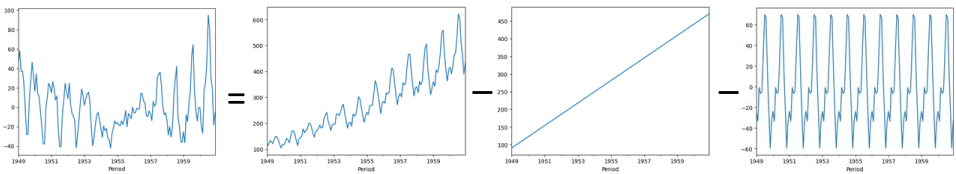
\includegraphics[width=0.5\linewidth]{img/TS_residuals.png}
    \caption{Enter Caption}
    \label{fig:12-lbl1}
\end{figure}

\subsubsection{Component-Based Normalizations}

\begin{itemize}
    \item \textbf{Detrend}:
    \begin{equation}
    Y' = Y - T
    \end{equation}
    
    \item \textbf{Deseasonalize}:
    \begin{equation}
    Y' = Y - S
    \end{equation}
    
    \item \textbf{Denoise}:
    \begin{equation}
    Y' = Y - R
    \end{equation}
\end{itemize}

\begin{figure}[h]
    \centering
    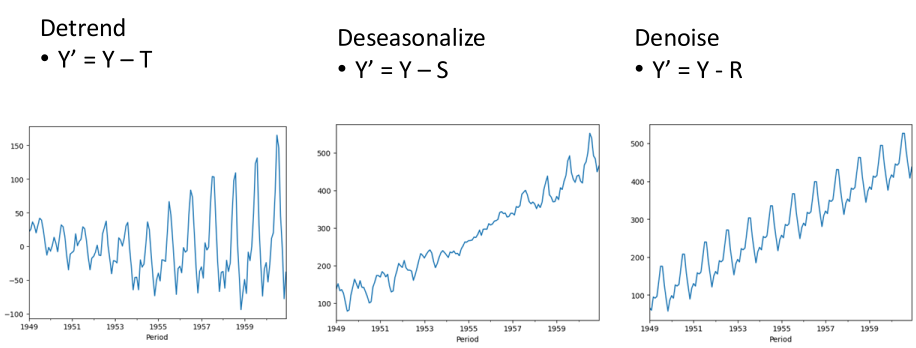
\includegraphics[width=0.5\linewidth]{img/component_based_normalizations.png}
    \caption{Enter Caption}
    \label{fig:12-lbl2}
\end{figure}